% -*- compile-command: "pdflatex --enable-write18 binomial-heap.tex" -*-
\documentclass{tufte-handout}

\usepackage{algo-activity}

\title{Algorithms: Binomial Heaps}
\date{}

\begin{document}

\maketitle

\begin{objective}
  Students will learn about binomial heaps and analyze their amortized running time.
\end{objective}

\begin{model*}{Binomial Trees}{binomial-trees}
  \begin{defn}
    A \term{binomial tree} of order $n$ (for $n \geq 0$) consists of a root
    node with $n$ subtrees. The leftmost subtree is of order $n-1$,
    the next subtree is of order $n-2$, and so forth, with the
    rightmost subtree being of order 0.
  \end{defn}

  The image below depicts a series of \emph{binomial trees} in
  increasing order. The leftmost tree is order 0, the next one is
  order 1, the third one is order 2, the fourth one is order 3, and
  the final tree is order 4.

  \begin{center}
  \begin{pgfpicture}
  \pgfpathrectangle{\pgfpointorigin}{\pgfqpoint{400.0000bp}{102.0000bp}}
  \pgfusepath{use as bounding box}
  \begin{pgfscope}
    \definecolor{fc}{rgb}{0.0000,0.0000,0.0000}
    \pgfsetfillcolor{fc}
    \pgfsetfillopacity{0.0000}
    \pgfsetlinewidth{0.8113bp}
    \definecolor{sc}{rgb}{0.0000,0.0000,0.0000}
    \pgfsetstrokecolor{sc}
    \pgfsetmiterjoin
    \pgfsetbuttcap
    \pgfpathqmoveto{400.0000bp}{5.7143bp}
    \pgfpathqcurveto{400.0000bp}{8.8702bp}{397.4416bp}{11.4286bp}{394.2857bp}{11.4286bp}
    \pgfpathqcurveto{391.1298bp}{11.4286bp}{388.5714bp}{8.8702bp}{388.5714bp}{5.7143bp}
    \pgfpathqcurveto{388.5714bp}{2.5584bp}{391.1298bp}{0.0000bp}{394.2857bp}{0.0000bp}
    \pgfpathqcurveto{397.4416bp}{0.0000bp}{400.0000bp}{2.5584bp}{400.0000bp}{5.7143bp}
    \pgfpathclose
    \pgfusepathqfillstroke
  \end{pgfscope}
  \begin{pgfscope}
    \definecolor{fc}{rgb}{0.0000,0.0000,0.0000}
    \pgfsetfillcolor{fc}
    \pgfsetfillopacity{0.0000}
    \pgfsetlinewidth{0.8113bp}
    \definecolor{sc}{rgb}{0.0000,0.0000,0.0000}
    \pgfsetstrokecolor{sc}
    \pgfsetmiterjoin
    \pgfsetbuttcap
    \pgfpathqmoveto{400.0000bp}{28.5714bp}
    \pgfpathqcurveto{400.0000bp}{31.7273bp}{397.4416bp}{34.2857bp}{394.2857bp}{34.2857bp}
    \pgfpathqcurveto{391.1298bp}{34.2857bp}{388.5714bp}{31.7273bp}{388.5714bp}{28.5714bp}
    \pgfpathqcurveto{388.5714bp}{25.4155bp}{391.1298bp}{22.8571bp}{394.2857bp}{22.8571bp}
    \pgfpathqcurveto{397.4416bp}{22.8571bp}{400.0000bp}{25.4155bp}{400.0000bp}{28.5714bp}
    \pgfpathclose
    \pgfusepathqfillstroke
  \end{pgfscope}
  \begin{pgfscope}
    \pgfsetlinewidth{0.8113bp}
    \definecolor{sc}{rgb}{0.0000,0.0000,0.0000}
    \pgfsetstrokecolor{sc}
    \pgfsetmiterjoin
    \pgfsetbuttcap
    \pgfpathqmoveto{394.2857bp}{22.8571bp}
    \pgfpathqlineto{394.2857bp}{11.4286bp}
    \pgfusepathqstroke
  \end{pgfscope}
  \begin{pgfscope}
    \definecolor{fc}{rgb}{0.0000,0.0000,0.0000}
    \pgfsetfillcolor{fc}
    \pgfusepathqfill
  \end{pgfscope}
  \begin{pgfscope}
    \definecolor{fc}{rgb}{0.0000,0.0000,0.0000}
    \pgfsetfillcolor{fc}
    \pgfusepathqfill
  \end{pgfscope}
  \begin{pgfscope}
    \definecolor{fc}{rgb}{0.0000,0.0000,0.0000}
    \pgfsetfillcolor{fc}
    \pgfusepathqfill
  \end{pgfscope}
  \begin{pgfscope}
    \definecolor{fc}{rgb}{0.0000,0.0000,0.0000}
    \pgfsetfillcolor{fc}
    \pgfusepathqfill
  \end{pgfscope}
  \begin{pgfscope}
    \definecolor{fc}{rgb}{0.0000,0.0000,0.0000}
    \pgfsetfillcolor{fc}
    \pgfsetfillopacity{0.0000}
    \pgfsetlinewidth{0.8113bp}
    \definecolor{sc}{rgb}{0.0000,0.0000,0.0000}
    \pgfsetstrokecolor{sc}
    \pgfsetmiterjoin
    \pgfsetbuttcap
    \pgfpathqmoveto{377.1429bp}{28.5714bp}
    \pgfpathqcurveto{377.1429bp}{31.7273bp}{374.5845bp}{34.2857bp}{371.4286bp}{34.2857bp}
    \pgfpathqcurveto{368.2727bp}{34.2857bp}{365.7143bp}{31.7273bp}{365.7143bp}{28.5714bp}
    \pgfpathqcurveto{365.7143bp}{25.4155bp}{368.2727bp}{22.8571bp}{371.4286bp}{22.8571bp}
    \pgfpathqcurveto{374.5845bp}{22.8571bp}{377.1429bp}{25.4155bp}{377.1429bp}{28.5714bp}
    \pgfpathclose
    \pgfusepathqfillstroke
  \end{pgfscope}
  \begin{pgfscope}
    \definecolor{fc}{rgb}{0.0000,0.0000,0.0000}
    \pgfsetfillcolor{fc}
    \pgfsetfillopacity{0.0000}
    \pgfsetlinewidth{0.8113bp}
    \definecolor{sc}{rgb}{0.0000,0.0000,0.0000}
    \pgfsetstrokecolor{sc}
    \pgfsetmiterjoin
    \pgfsetbuttcap
    \pgfpathqmoveto{377.1429bp}{51.4286bp}
    \pgfpathqcurveto{377.1429bp}{54.5845bp}{374.5845bp}{57.1429bp}{371.4286bp}{57.1429bp}
    \pgfpathqcurveto{368.2727bp}{57.1429bp}{365.7143bp}{54.5845bp}{365.7143bp}{51.4286bp}
    \pgfpathqcurveto{365.7143bp}{48.2727bp}{368.2727bp}{45.7143bp}{371.4286bp}{45.7143bp}
    \pgfpathqcurveto{374.5845bp}{45.7143bp}{377.1429bp}{48.2727bp}{377.1429bp}{51.4286bp}
    \pgfpathclose
    \pgfusepathqfillstroke
  \end{pgfscope}
  \begin{pgfscope}
    \pgfsetlinewidth{0.8113bp}
    \definecolor{sc}{rgb}{0.0000,0.0000,0.0000}
    \pgfsetstrokecolor{sc}
    \pgfsetmiterjoin
    \pgfsetbuttcap
    \pgfpathqmoveto{375.4692bp}{47.3880bp}
    \pgfpathqlineto{390.2451bp}{32.6120bp}
    \pgfusepathqstroke
  \end{pgfscope}
  \begin{pgfscope}
    \definecolor{fc}{rgb}{0.0000,0.0000,0.0000}
    \pgfsetfillcolor{fc}
    \pgfusepathqfill
  \end{pgfscope}
  \begin{pgfscope}
    \definecolor{fc}{rgb}{0.0000,0.0000,0.0000}
    \pgfsetfillcolor{fc}
    \pgfusepathqfill
  \end{pgfscope}
  \begin{pgfscope}
    \definecolor{fc}{rgb}{0.0000,0.0000,0.0000}
    \pgfsetfillcolor{fc}
    \pgfusepathqfill
  \end{pgfscope}
  \begin{pgfscope}
    \definecolor{fc}{rgb}{0.0000,0.0000,0.0000}
    \pgfsetfillcolor{fc}
    \pgfusepathqfill
  \end{pgfscope}
  \begin{pgfscope}
    \pgfsetlinewidth{0.8113bp}
    \definecolor{sc}{rgb}{0.0000,0.0000,0.0000}
    \pgfsetstrokecolor{sc}
    \pgfsetmiterjoin
    \pgfsetbuttcap
    \pgfpathqmoveto{371.4286bp}{45.7143bp}
    \pgfpathqlineto{371.4286bp}{34.2857bp}
    \pgfusepathqstroke
  \end{pgfscope}
  \begin{pgfscope}
    \definecolor{fc}{rgb}{0.0000,0.0000,0.0000}
    \pgfsetfillcolor{fc}
    \pgfusepathqfill
  \end{pgfscope}
  \begin{pgfscope}
    \definecolor{fc}{rgb}{0.0000,0.0000,0.0000}
    \pgfsetfillcolor{fc}
    \pgfusepathqfill
  \end{pgfscope}
  \begin{pgfscope}
    \definecolor{fc}{rgb}{0.0000,0.0000,0.0000}
    \pgfsetfillcolor{fc}
    \pgfusepathqfill
  \end{pgfscope}
  \begin{pgfscope}
    \definecolor{fc}{rgb}{0.0000,0.0000,0.0000}
    \pgfsetfillcolor{fc}
    \pgfusepathqfill
  \end{pgfscope}
  \begin{pgfscope}
    \definecolor{fc}{rgb}{0.0000,0.0000,0.0000}
    \pgfsetfillcolor{fc}
    \pgfsetfillopacity{0.0000}
    \pgfsetlinewidth{0.8113bp}
    \definecolor{sc}{rgb}{0.0000,0.0000,0.0000}
    \pgfsetstrokecolor{sc}
    \pgfsetmiterjoin
    \pgfsetbuttcap
    \pgfpathqmoveto{354.2857bp}{28.5714bp}
    \pgfpathqcurveto{354.2857bp}{31.7273bp}{351.7273bp}{34.2857bp}{348.5714bp}{34.2857bp}
    \pgfpathqcurveto{345.4155bp}{34.2857bp}{342.8571bp}{31.7273bp}{342.8571bp}{28.5714bp}
    \pgfpathqcurveto{342.8571bp}{25.4155bp}{345.4155bp}{22.8571bp}{348.5714bp}{22.8571bp}
    \pgfpathqcurveto{351.7273bp}{22.8571bp}{354.2857bp}{25.4155bp}{354.2857bp}{28.5714bp}
    \pgfpathclose
    \pgfusepathqfillstroke
  \end{pgfscope}
  \begin{pgfscope}
    \definecolor{fc}{rgb}{0.0000,0.0000,0.0000}
    \pgfsetfillcolor{fc}
    \pgfsetfillopacity{0.0000}
    \pgfsetlinewidth{0.8113bp}
    \definecolor{sc}{rgb}{0.0000,0.0000,0.0000}
    \pgfsetstrokecolor{sc}
    \pgfsetmiterjoin
    \pgfsetbuttcap
    \pgfpathqmoveto{354.2857bp}{51.4286bp}
    \pgfpathqcurveto{354.2857bp}{54.5845bp}{351.7273bp}{57.1429bp}{348.5714bp}{57.1429bp}
    \pgfpathqcurveto{345.4155bp}{57.1429bp}{342.8571bp}{54.5845bp}{342.8571bp}{51.4286bp}
    \pgfpathqcurveto{342.8571bp}{48.2727bp}{345.4155bp}{45.7143bp}{348.5714bp}{45.7143bp}
    \pgfpathqcurveto{351.7273bp}{45.7143bp}{354.2857bp}{48.2727bp}{354.2857bp}{51.4286bp}
    \pgfpathclose
    \pgfusepathqfillstroke
  \end{pgfscope}
  \begin{pgfscope}
    \pgfsetlinewidth{0.8113bp}
    \definecolor{sc}{rgb}{0.0000,0.0000,0.0000}
    \pgfsetstrokecolor{sc}
    \pgfsetmiterjoin
    \pgfsetbuttcap
    \pgfpathqmoveto{348.5714bp}{45.7143bp}
    \pgfpathqlineto{348.5714bp}{34.2857bp}
    \pgfusepathqstroke
  \end{pgfscope}
  \begin{pgfscope}
    \definecolor{fc}{rgb}{0.0000,0.0000,0.0000}
    \pgfsetfillcolor{fc}
    \pgfusepathqfill
  \end{pgfscope}
  \begin{pgfscope}
    \definecolor{fc}{rgb}{0.0000,0.0000,0.0000}
    \pgfsetfillcolor{fc}
    \pgfusepathqfill
  \end{pgfscope}
  \begin{pgfscope}
    \definecolor{fc}{rgb}{0.0000,0.0000,0.0000}
    \pgfsetfillcolor{fc}
    \pgfusepathqfill
  \end{pgfscope}
  \begin{pgfscope}
    \definecolor{fc}{rgb}{0.0000,0.0000,0.0000}
    \pgfsetfillcolor{fc}
    \pgfusepathqfill
  \end{pgfscope}
  \begin{pgfscope}
    \definecolor{fc}{rgb}{0.0000,0.0000,0.0000}
    \pgfsetfillcolor{fc}
    \pgfsetfillopacity{0.0000}
    \pgfsetlinewidth{0.8113bp}
    \definecolor{sc}{rgb}{0.0000,0.0000,0.0000}
    \pgfsetstrokecolor{sc}
    \pgfsetmiterjoin
    \pgfsetbuttcap
    \pgfpathqmoveto{331.4286bp}{51.4286bp}
    \pgfpathqcurveto{331.4286bp}{54.5845bp}{328.8702bp}{57.1429bp}{325.7143bp}{57.1429bp}
    \pgfpathqcurveto{322.5584bp}{57.1429bp}{320.0000bp}{54.5845bp}{320.0000bp}{51.4286bp}
    \pgfpathqcurveto{320.0000bp}{48.2727bp}{322.5584bp}{45.7143bp}{325.7143bp}{45.7143bp}
    \pgfpathqcurveto{328.8702bp}{45.7143bp}{331.4286bp}{48.2727bp}{331.4286bp}{51.4286bp}
    \pgfpathclose
    \pgfusepathqfillstroke
  \end{pgfscope}
  \begin{pgfscope}
    \definecolor{fc}{rgb}{0.0000,0.0000,0.0000}
    \pgfsetfillcolor{fc}
    \pgfsetfillopacity{0.0000}
    \pgfsetlinewidth{0.8113bp}
    \definecolor{sc}{rgb}{0.0000,0.0000,0.0000}
    \pgfsetstrokecolor{sc}
    \pgfsetmiterjoin
    \pgfsetbuttcap
    \pgfpathqmoveto{331.4286bp}{74.2857bp}
    \pgfpathqcurveto{331.4286bp}{77.4416bp}{328.8702bp}{80.0000bp}{325.7143bp}{80.0000bp}
    \pgfpathqcurveto{322.5584bp}{80.0000bp}{320.0000bp}{77.4416bp}{320.0000bp}{74.2857bp}
    \pgfpathqcurveto{320.0000bp}{71.1298bp}{322.5584bp}{68.5714bp}{325.7143bp}{68.5714bp}
    \pgfpathqcurveto{328.8702bp}{68.5714bp}{331.4286bp}{71.1298bp}{331.4286bp}{74.2857bp}
    \pgfpathclose
    \pgfusepathqfillstroke
  \end{pgfscope}
  \begin{pgfscope}
    \pgfsetlinewidth{0.8113bp}
    \definecolor{sc}{rgb}{0.0000,0.0000,0.0000}
    \pgfsetstrokecolor{sc}
    \pgfsetmiterjoin
    \pgfsetbuttcap
    \pgfpathqmoveto{330.8264bp}{71.7296bp}
    \pgfpathqlineto{366.3164bp}{53.9846bp}
    \pgfusepathqstroke
  \end{pgfscope}
  \begin{pgfscope}
    \definecolor{fc}{rgb}{0.0000,0.0000,0.0000}
    \pgfsetfillcolor{fc}
    \pgfusepathqfill
  \end{pgfscope}
  \begin{pgfscope}
    \definecolor{fc}{rgb}{0.0000,0.0000,0.0000}
    \pgfsetfillcolor{fc}
    \pgfusepathqfill
  \end{pgfscope}
  \begin{pgfscope}
    \definecolor{fc}{rgb}{0.0000,0.0000,0.0000}
    \pgfsetfillcolor{fc}
    \pgfusepathqfill
  \end{pgfscope}
  \begin{pgfscope}
    \definecolor{fc}{rgb}{0.0000,0.0000,0.0000}
    \pgfsetfillcolor{fc}
    \pgfusepathqfill
  \end{pgfscope}
  \begin{pgfscope}
    \pgfsetlinewidth{0.8113bp}
    \definecolor{sc}{rgb}{0.0000,0.0000,0.0000}
    \pgfsetstrokecolor{sc}
    \pgfsetmiterjoin
    \pgfsetbuttcap
    \pgfpathqmoveto{329.7549bp}{70.2451bp}
    \pgfpathqlineto{344.5308bp}{55.4692bp}
    \pgfusepathqstroke
  \end{pgfscope}
  \begin{pgfscope}
    \definecolor{fc}{rgb}{0.0000,0.0000,0.0000}
    \pgfsetfillcolor{fc}
    \pgfusepathqfill
  \end{pgfscope}
  \begin{pgfscope}
    \definecolor{fc}{rgb}{0.0000,0.0000,0.0000}
    \pgfsetfillcolor{fc}
    \pgfusepathqfill
  \end{pgfscope}
  \begin{pgfscope}
    \definecolor{fc}{rgb}{0.0000,0.0000,0.0000}
    \pgfsetfillcolor{fc}
    \pgfusepathqfill
  \end{pgfscope}
  \begin{pgfscope}
    \definecolor{fc}{rgb}{0.0000,0.0000,0.0000}
    \pgfsetfillcolor{fc}
    \pgfusepathqfill
  \end{pgfscope}
  \begin{pgfscope}
    \pgfsetlinewidth{0.8113bp}
    \definecolor{sc}{rgb}{0.0000,0.0000,0.0000}
    \pgfsetstrokecolor{sc}
    \pgfsetmiterjoin
    \pgfsetbuttcap
    \pgfpathqmoveto{325.7143bp}{68.5714bp}
    \pgfpathqlineto{325.7143bp}{57.1429bp}
    \pgfusepathqstroke
  \end{pgfscope}
  \begin{pgfscope}
    \definecolor{fc}{rgb}{0.0000,0.0000,0.0000}
    \pgfsetfillcolor{fc}
    \pgfusepathqfill
  \end{pgfscope}
  \begin{pgfscope}
    \definecolor{fc}{rgb}{0.0000,0.0000,0.0000}
    \pgfsetfillcolor{fc}
    \pgfusepathqfill
  \end{pgfscope}
  \begin{pgfscope}
    \definecolor{fc}{rgb}{0.0000,0.0000,0.0000}
    \pgfsetfillcolor{fc}
    \pgfusepathqfill
  \end{pgfscope}
  \begin{pgfscope}
    \definecolor{fc}{rgb}{0.0000,0.0000,0.0000}
    \pgfsetfillcolor{fc}
    \pgfusepathqfill
  \end{pgfscope}
  \begin{pgfscope}
    \definecolor{fc}{rgb}{0.0000,0.0000,0.0000}
    \pgfsetfillcolor{fc}
    \pgfsetfillopacity{0.0000}
    \pgfsetlinewidth{0.8113bp}
    \definecolor{sc}{rgb}{0.0000,0.0000,0.0000}
    \pgfsetstrokecolor{sc}
    \pgfsetmiterjoin
    \pgfsetbuttcap
    \pgfpathqmoveto{308.5714bp}{28.5714bp}
    \pgfpathqcurveto{308.5714bp}{31.7273bp}{306.0131bp}{34.2857bp}{302.8571bp}{34.2857bp}
    \pgfpathqcurveto{299.7012bp}{34.2857bp}{297.1429bp}{31.7273bp}{297.1429bp}{28.5714bp}
    \pgfpathqcurveto{297.1429bp}{25.4155bp}{299.7012bp}{22.8571bp}{302.8571bp}{22.8571bp}
    \pgfpathqcurveto{306.0131bp}{22.8571bp}{308.5714bp}{25.4155bp}{308.5714bp}{28.5714bp}
    \pgfpathclose
    \pgfusepathqfillstroke
  \end{pgfscope}
  \begin{pgfscope}
    \definecolor{fc}{rgb}{0.0000,0.0000,0.0000}
    \pgfsetfillcolor{fc}
    \pgfsetfillopacity{0.0000}
    \pgfsetlinewidth{0.8113bp}
    \definecolor{sc}{rgb}{0.0000,0.0000,0.0000}
    \pgfsetstrokecolor{sc}
    \pgfsetmiterjoin
    \pgfsetbuttcap
    \pgfpathqmoveto{308.5714bp}{51.4286bp}
    \pgfpathqcurveto{308.5714bp}{54.5845bp}{306.0131bp}{57.1429bp}{302.8571bp}{57.1429bp}
    \pgfpathqcurveto{299.7012bp}{57.1429bp}{297.1429bp}{54.5845bp}{297.1429bp}{51.4286bp}
    \pgfpathqcurveto{297.1429bp}{48.2727bp}{299.7012bp}{45.7143bp}{302.8571bp}{45.7143bp}
    \pgfpathqcurveto{306.0131bp}{45.7143bp}{308.5714bp}{48.2727bp}{308.5714bp}{51.4286bp}
    \pgfpathclose
    \pgfusepathqfillstroke
  \end{pgfscope}
  \begin{pgfscope}
    \pgfsetlinewidth{0.8113bp}
    \definecolor{sc}{rgb}{0.0000,0.0000,0.0000}
    \pgfsetstrokecolor{sc}
    \pgfsetmiterjoin
    \pgfsetbuttcap
    \pgfpathqmoveto{302.8571bp}{45.7143bp}
    \pgfpathqlineto{302.8571bp}{34.2857bp}
    \pgfusepathqstroke
  \end{pgfscope}
  \begin{pgfscope}
    \definecolor{fc}{rgb}{0.0000,0.0000,0.0000}
    \pgfsetfillcolor{fc}
    \pgfusepathqfill
  \end{pgfscope}
  \begin{pgfscope}
    \definecolor{fc}{rgb}{0.0000,0.0000,0.0000}
    \pgfsetfillcolor{fc}
    \pgfusepathqfill
  \end{pgfscope}
  \begin{pgfscope}
    \definecolor{fc}{rgb}{0.0000,0.0000,0.0000}
    \pgfsetfillcolor{fc}
    \pgfusepathqfill
  \end{pgfscope}
  \begin{pgfscope}
    \definecolor{fc}{rgb}{0.0000,0.0000,0.0000}
    \pgfsetfillcolor{fc}
    \pgfusepathqfill
  \end{pgfscope}
  \begin{pgfscope}
    \definecolor{fc}{rgb}{0.0000,0.0000,0.0000}
    \pgfsetfillcolor{fc}
    \pgfsetfillopacity{0.0000}
    \pgfsetlinewidth{0.8113bp}
    \definecolor{sc}{rgb}{0.0000,0.0000,0.0000}
    \pgfsetstrokecolor{sc}
    \pgfsetmiterjoin
    \pgfsetbuttcap
    \pgfpathqmoveto{285.7143bp}{51.4286bp}
    \pgfpathqcurveto{285.7143bp}{54.5845bp}{283.1559bp}{57.1429bp}{280.0000bp}{57.1429bp}
    \pgfpathqcurveto{276.8441bp}{57.1429bp}{274.2857bp}{54.5845bp}{274.2857bp}{51.4286bp}
    \pgfpathqcurveto{274.2857bp}{48.2727bp}{276.8441bp}{45.7143bp}{280.0000bp}{45.7143bp}
    \pgfpathqcurveto{283.1559bp}{45.7143bp}{285.7143bp}{48.2727bp}{285.7143bp}{51.4286bp}
    \pgfpathclose
    \pgfusepathqfillstroke
  \end{pgfscope}
  \begin{pgfscope}
    \definecolor{fc}{rgb}{0.0000,0.0000,0.0000}
    \pgfsetfillcolor{fc}
    \pgfsetfillopacity{0.0000}
    \pgfsetlinewidth{0.8113bp}
    \definecolor{sc}{rgb}{0.0000,0.0000,0.0000}
    \pgfsetstrokecolor{sc}
    \pgfsetmiterjoin
    \pgfsetbuttcap
    \pgfpathqmoveto{285.7143bp}{74.2857bp}
    \pgfpathqcurveto{285.7143bp}{77.4416bp}{283.1559bp}{80.0000bp}{280.0000bp}{80.0000bp}
    \pgfpathqcurveto{276.8441bp}{80.0000bp}{274.2857bp}{77.4416bp}{274.2857bp}{74.2857bp}
    \pgfpathqcurveto{274.2857bp}{71.1298bp}{276.8441bp}{68.5714bp}{280.0000bp}{68.5714bp}
    \pgfpathqcurveto{283.1559bp}{68.5714bp}{285.7143bp}{71.1298bp}{285.7143bp}{74.2857bp}
    \pgfpathclose
    \pgfusepathqfillstroke
  \end{pgfscope}
  \begin{pgfscope}
    \pgfsetlinewidth{0.8113bp}
    \definecolor{sc}{rgb}{0.0000,0.0000,0.0000}
    \pgfsetstrokecolor{sc}
    \pgfsetmiterjoin
    \pgfsetbuttcap
    \pgfpathqmoveto{284.0406bp}{70.2451bp}
    \pgfpathqlineto{298.8165bp}{55.4692bp}
    \pgfusepathqstroke
  \end{pgfscope}
  \begin{pgfscope}
    \definecolor{fc}{rgb}{0.0000,0.0000,0.0000}
    \pgfsetfillcolor{fc}
    \pgfusepathqfill
  \end{pgfscope}
  \begin{pgfscope}
    \definecolor{fc}{rgb}{0.0000,0.0000,0.0000}
    \pgfsetfillcolor{fc}
    \pgfusepathqfill
  \end{pgfscope}
  \begin{pgfscope}
    \definecolor{fc}{rgb}{0.0000,0.0000,0.0000}
    \pgfsetfillcolor{fc}
    \pgfusepathqfill
  \end{pgfscope}
  \begin{pgfscope}
    \definecolor{fc}{rgb}{0.0000,0.0000,0.0000}
    \pgfsetfillcolor{fc}
    \pgfusepathqfill
  \end{pgfscope}
  \begin{pgfscope}
    \pgfsetlinewidth{0.8113bp}
    \definecolor{sc}{rgb}{0.0000,0.0000,0.0000}
    \pgfsetstrokecolor{sc}
    \pgfsetmiterjoin
    \pgfsetbuttcap
    \pgfpathqmoveto{280.0000bp}{68.5714bp}
    \pgfpathqlineto{280.0000bp}{57.1429bp}
    \pgfusepathqstroke
  \end{pgfscope}
  \begin{pgfscope}
    \definecolor{fc}{rgb}{0.0000,0.0000,0.0000}
    \pgfsetfillcolor{fc}
    \pgfusepathqfill
  \end{pgfscope}
  \begin{pgfscope}
    \definecolor{fc}{rgb}{0.0000,0.0000,0.0000}
    \pgfsetfillcolor{fc}
    \pgfusepathqfill
  \end{pgfscope}
  \begin{pgfscope}
    \definecolor{fc}{rgb}{0.0000,0.0000,0.0000}
    \pgfsetfillcolor{fc}
    \pgfusepathqfill
  \end{pgfscope}
  \begin{pgfscope}
    \definecolor{fc}{rgb}{0.0000,0.0000,0.0000}
    \pgfsetfillcolor{fc}
    \pgfusepathqfill
  \end{pgfscope}
  \begin{pgfscope}
    \definecolor{fc}{rgb}{0.0000,0.0000,0.0000}
    \pgfsetfillcolor{fc}
    \pgfsetfillopacity{0.0000}
    \pgfsetlinewidth{0.8113bp}
    \definecolor{sc}{rgb}{0.0000,0.0000,0.0000}
    \pgfsetstrokecolor{sc}
    \pgfsetmiterjoin
    \pgfsetbuttcap
    \pgfpathqmoveto{262.8571bp}{51.4286bp}
    \pgfpathqcurveto{262.8571bp}{54.5845bp}{260.2988bp}{57.1429bp}{257.1429bp}{57.1429bp}
    \pgfpathqcurveto{253.9869bp}{57.1429bp}{251.4286bp}{54.5845bp}{251.4286bp}{51.4286bp}
    \pgfpathqcurveto{251.4286bp}{48.2727bp}{253.9869bp}{45.7143bp}{257.1429bp}{45.7143bp}
    \pgfpathqcurveto{260.2988bp}{45.7143bp}{262.8571bp}{48.2727bp}{262.8571bp}{51.4286bp}
    \pgfpathclose
    \pgfusepathqfillstroke
  \end{pgfscope}
  \begin{pgfscope}
    \definecolor{fc}{rgb}{0.0000,0.0000,0.0000}
    \pgfsetfillcolor{fc}
    \pgfsetfillopacity{0.0000}
    \pgfsetlinewidth{0.8113bp}
    \definecolor{sc}{rgb}{0.0000,0.0000,0.0000}
    \pgfsetstrokecolor{sc}
    \pgfsetmiterjoin
    \pgfsetbuttcap
    \pgfpathqmoveto{262.8571bp}{74.2857bp}
    \pgfpathqcurveto{262.8571bp}{77.4416bp}{260.2988bp}{80.0000bp}{257.1429bp}{80.0000bp}
    \pgfpathqcurveto{253.9869bp}{80.0000bp}{251.4286bp}{77.4416bp}{251.4286bp}{74.2857bp}
    \pgfpathqcurveto{251.4286bp}{71.1298bp}{253.9869bp}{68.5714bp}{257.1429bp}{68.5714bp}
    \pgfpathqcurveto{260.2988bp}{68.5714bp}{262.8571bp}{71.1298bp}{262.8571bp}{74.2857bp}
    \pgfpathclose
    \pgfusepathqfillstroke
  \end{pgfscope}
  \begin{pgfscope}
    \pgfsetlinewidth{0.8113bp}
    \definecolor{sc}{rgb}{0.0000,0.0000,0.0000}
    \pgfsetstrokecolor{sc}
    \pgfsetmiterjoin
    \pgfsetbuttcap
    \pgfpathqmoveto{257.1429bp}{68.5714bp}
    \pgfpathqlineto{257.1429bp}{57.1429bp}
    \pgfusepathqstroke
  \end{pgfscope}
  \begin{pgfscope}
    \definecolor{fc}{rgb}{0.0000,0.0000,0.0000}
    \pgfsetfillcolor{fc}
    \pgfusepathqfill
  \end{pgfscope}
  \begin{pgfscope}
    \definecolor{fc}{rgb}{0.0000,0.0000,0.0000}
    \pgfsetfillcolor{fc}
    \pgfusepathqfill
  \end{pgfscope}
  \begin{pgfscope}
    \definecolor{fc}{rgb}{0.0000,0.0000,0.0000}
    \pgfsetfillcolor{fc}
    \pgfusepathqfill
  \end{pgfscope}
  \begin{pgfscope}
    \definecolor{fc}{rgb}{0.0000,0.0000,0.0000}
    \pgfsetfillcolor{fc}
    \pgfusepathqfill
  \end{pgfscope}
  \begin{pgfscope}
    \definecolor{fc}{rgb}{0.0000,0.0000,0.0000}
    \pgfsetfillcolor{fc}
    \pgfsetfillopacity{0.0000}
    \pgfsetlinewidth{0.8113bp}
    \definecolor{sc}{rgb}{0.0000,0.0000,0.0000}
    \pgfsetstrokecolor{sc}
    \pgfsetmiterjoin
    \pgfsetbuttcap
    \pgfpathqmoveto{240.0000bp}{74.2857bp}
    \pgfpathqcurveto{240.0000bp}{77.4416bp}{237.4416bp}{80.0000bp}{234.2857bp}{80.0000bp}
    \pgfpathqcurveto{231.1298bp}{80.0000bp}{228.5714bp}{77.4416bp}{228.5714bp}{74.2857bp}
    \pgfpathqcurveto{228.5714bp}{71.1298bp}{231.1298bp}{68.5714bp}{234.2857bp}{68.5714bp}
    \pgfpathqcurveto{237.4416bp}{68.5714bp}{240.0000bp}{71.1298bp}{240.0000bp}{74.2857bp}
    \pgfpathclose
    \pgfusepathqfillstroke
  \end{pgfscope}
  \begin{pgfscope}
    \definecolor{fc}{rgb}{0.0000,0.0000,0.0000}
    \pgfsetfillcolor{fc}
    \pgfsetfillopacity{0.0000}
    \pgfsetlinewidth{0.8113bp}
    \definecolor{sc}{rgb}{0.0000,0.0000,0.0000}
    \pgfsetstrokecolor{sc}
    \pgfsetmiterjoin
    \pgfsetbuttcap
    \pgfpathqmoveto{240.0000bp}{97.1429bp}
    \pgfpathqcurveto{240.0000bp}{100.2988bp}{237.4416bp}{102.8571bp}{234.2857bp}{102.8571bp}
    \pgfpathqcurveto{231.1298bp}{102.8571bp}{228.5714bp}{100.2988bp}{228.5714bp}{97.1429bp}
    \pgfpathqcurveto{228.5714bp}{93.9869bp}{231.1298bp}{91.4286bp}{234.2857bp}{91.4286bp}
    \pgfpathqcurveto{237.4416bp}{91.4286bp}{240.0000bp}{93.9869bp}{240.0000bp}{97.1429bp}
    \pgfpathclose
    \pgfusepathqfillstroke
  \end{pgfscope}
  \begin{pgfscope}
    \pgfsetlinewidth{0.8113bp}
    \definecolor{sc}{rgb}{0.0000,0.0000,0.0000}
    \pgfsetstrokecolor{sc}
    \pgfsetmiterjoin
    \pgfsetbuttcap
    \pgfpathqmoveto{239.8307bp}{95.7566bp}
    \pgfpathqlineto{320.1693bp}{75.6720bp}
    \pgfusepathqstroke
  \end{pgfscope}
  \begin{pgfscope}
    \definecolor{fc}{rgb}{0.0000,0.0000,0.0000}
    \pgfsetfillcolor{fc}
    \pgfusepathqfill
  \end{pgfscope}
  \begin{pgfscope}
    \definecolor{fc}{rgb}{0.0000,0.0000,0.0000}
    \pgfsetfillcolor{fc}
    \pgfusepathqfill
  \end{pgfscope}
  \begin{pgfscope}
    \definecolor{fc}{rgb}{0.0000,0.0000,0.0000}
    \pgfsetfillcolor{fc}
    \pgfusepathqfill
  \end{pgfscope}
  \begin{pgfscope}
    \definecolor{fc}{rgb}{0.0000,0.0000,0.0000}
    \pgfsetfillcolor{fc}
    \pgfusepathqfill
  \end{pgfscope}
  \begin{pgfscope}
    \pgfsetlinewidth{0.8113bp}
    \definecolor{sc}{rgb}{0.0000,0.0000,0.0000}
    \pgfsetstrokecolor{sc}
    \pgfsetmiterjoin
    \pgfsetbuttcap
    \pgfpathqmoveto{239.3978bp}{94.5868bp}
    \pgfpathqlineto{274.8879bp}{76.8418bp}
    \pgfusepathqstroke
  \end{pgfscope}
  \begin{pgfscope}
    \definecolor{fc}{rgb}{0.0000,0.0000,0.0000}
    \pgfsetfillcolor{fc}
    \pgfusepathqfill
  \end{pgfscope}
  \begin{pgfscope}
    \definecolor{fc}{rgb}{0.0000,0.0000,0.0000}
    \pgfsetfillcolor{fc}
    \pgfusepathqfill
  \end{pgfscope}
  \begin{pgfscope}
    \definecolor{fc}{rgb}{0.0000,0.0000,0.0000}
    \pgfsetfillcolor{fc}
    \pgfusepathqfill
  \end{pgfscope}
  \begin{pgfscope}
    \definecolor{fc}{rgb}{0.0000,0.0000,0.0000}
    \pgfsetfillcolor{fc}
    \pgfusepathqfill
  \end{pgfscope}
  \begin{pgfscope}
    \pgfsetlinewidth{0.8113bp}
    \definecolor{sc}{rgb}{0.0000,0.0000,0.0000}
    \pgfsetstrokecolor{sc}
    \pgfsetmiterjoin
    \pgfsetbuttcap
    \pgfpathqmoveto{238.3263bp}{93.1022bp}
    \pgfpathqlineto{253.1022bp}{78.3263bp}
    \pgfusepathqstroke
  \end{pgfscope}
  \begin{pgfscope}
    \definecolor{fc}{rgb}{0.0000,0.0000,0.0000}
    \pgfsetfillcolor{fc}
    \pgfusepathqfill
  \end{pgfscope}
  \begin{pgfscope}
    \definecolor{fc}{rgb}{0.0000,0.0000,0.0000}
    \pgfsetfillcolor{fc}
    \pgfusepathqfill
  \end{pgfscope}
  \begin{pgfscope}
    \definecolor{fc}{rgb}{0.0000,0.0000,0.0000}
    \pgfsetfillcolor{fc}
    \pgfusepathqfill
  \end{pgfscope}
  \begin{pgfscope}
    \definecolor{fc}{rgb}{0.0000,0.0000,0.0000}
    \pgfsetfillcolor{fc}
    \pgfusepathqfill
  \end{pgfscope}
  \begin{pgfscope}
    \pgfsetlinewidth{0.8113bp}
    \definecolor{sc}{rgb}{0.0000,0.0000,0.0000}
    \pgfsetstrokecolor{sc}
    \pgfsetmiterjoin
    \pgfsetbuttcap
    \pgfpathqmoveto{234.2857bp}{91.4286bp}
    \pgfpathqlineto{234.2857bp}{80.0000bp}
    \pgfusepathqstroke
  \end{pgfscope}
  \begin{pgfscope}
    \definecolor{fc}{rgb}{0.0000,0.0000,0.0000}
    \pgfsetfillcolor{fc}
    \pgfusepathqfill
  \end{pgfscope}
  \begin{pgfscope}
    \definecolor{fc}{rgb}{0.0000,0.0000,0.0000}
    \pgfsetfillcolor{fc}
    \pgfusepathqfill
  \end{pgfscope}
  \begin{pgfscope}
    \definecolor{fc}{rgb}{0.0000,0.0000,0.0000}
    \pgfsetfillcolor{fc}
    \pgfusepathqfill
  \end{pgfscope}
  \begin{pgfscope}
    \definecolor{fc}{rgb}{0.0000,0.0000,0.0000}
    \pgfsetfillcolor{fc}
    \pgfusepathqfill
  \end{pgfscope}
  \begin{pgfscope}
    \definecolor{fc}{rgb}{0.0000,0.0000,0.0000}
    \pgfsetfillcolor{fc}
    \pgfsetfillopacity{0.0000}
    \pgfsetlinewidth{0.8113bp}
    \definecolor{sc}{rgb}{0.0000,0.0000,0.0000}
    \pgfsetstrokecolor{sc}
    \pgfsetmiterjoin
    \pgfsetbuttcap
    \pgfpathqmoveto{205.7143bp}{28.5714bp}
    \pgfpathqcurveto{205.7143bp}{31.7273bp}{203.1559bp}{34.2857bp}{200.0000bp}{34.2857bp}
    \pgfpathqcurveto{196.8441bp}{34.2857bp}{194.2857bp}{31.7273bp}{194.2857bp}{28.5714bp}
    \pgfpathqcurveto{194.2857bp}{25.4155bp}{196.8441bp}{22.8571bp}{200.0000bp}{22.8571bp}
    \pgfpathqcurveto{203.1559bp}{22.8571bp}{205.7143bp}{25.4155bp}{205.7143bp}{28.5714bp}
    \pgfpathclose
    \pgfusepathqfillstroke
  \end{pgfscope}
  \begin{pgfscope}
    \definecolor{fc}{rgb}{0.0000,0.0000,0.0000}
    \pgfsetfillcolor{fc}
    \pgfsetfillopacity{0.0000}
    \pgfsetlinewidth{0.8113bp}
    \definecolor{sc}{rgb}{0.0000,0.0000,0.0000}
    \pgfsetstrokecolor{sc}
    \pgfsetmiterjoin
    \pgfsetbuttcap
    \pgfpathqmoveto{205.7143bp}{51.4286bp}
    \pgfpathqcurveto{205.7143bp}{54.5845bp}{203.1559bp}{57.1429bp}{200.0000bp}{57.1429bp}
    \pgfpathqcurveto{196.8441bp}{57.1429bp}{194.2857bp}{54.5845bp}{194.2857bp}{51.4286bp}
    \pgfpathqcurveto{194.2857bp}{48.2727bp}{196.8441bp}{45.7143bp}{200.0000bp}{45.7143bp}
    \pgfpathqcurveto{203.1559bp}{45.7143bp}{205.7143bp}{48.2727bp}{205.7143bp}{51.4286bp}
    \pgfpathclose
    \pgfusepathqfillstroke
  \end{pgfscope}
  \begin{pgfscope}
    \pgfsetlinewidth{0.8113bp}
    \definecolor{sc}{rgb}{0.0000,0.0000,0.0000}
    \pgfsetstrokecolor{sc}
    \pgfsetmiterjoin
    \pgfsetbuttcap
    \pgfpathqmoveto{200.0000bp}{45.7143bp}
    \pgfpathqlineto{200.0000bp}{34.2857bp}
    \pgfusepathqstroke
  \end{pgfscope}
  \begin{pgfscope}
    \definecolor{fc}{rgb}{0.0000,0.0000,0.0000}
    \pgfsetfillcolor{fc}
    \pgfusepathqfill
  \end{pgfscope}
  \begin{pgfscope}
    \definecolor{fc}{rgb}{0.0000,0.0000,0.0000}
    \pgfsetfillcolor{fc}
    \pgfusepathqfill
  \end{pgfscope}
  \begin{pgfscope}
    \definecolor{fc}{rgb}{0.0000,0.0000,0.0000}
    \pgfsetfillcolor{fc}
    \pgfusepathqfill
  \end{pgfscope}
  \begin{pgfscope}
    \definecolor{fc}{rgb}{0.0000,0.0000,0.0000}
    \pgfsetfillcolor{fc}
    \pgfusepathqfill
  \end{pgfscope}
  \begin{pgfscope}
    \definecolor{fc}{rgb}{0.0000,0.0000,0.0000}
    \pgfsetfillcolor{fc}
    \pgfsetfillopacity{0.0000}
    \pgfsetlinewidth{0.8113bp}
    \definecolor{sc}{rgb}{0.0000,0.0000,0.0000}
    \pgfsetstrokecolor{sc}
    \pgfsetmiterjoin
    \pgfsetbuttcap
    \pgfpathqmoveto{182.8571bp}{51.4286bp}
    \pgfpathqcurveto{182.8571bp}{54.5845bp}{180.2988bp}{57.1429bp}{177.1429bp}{57.1429bp}
    \pgfpathqcurveto{173.9869bp}{57.1429bp}{171.4286bp}{54.5845bp}{171.4286bp}{51.4286bp}
    \pgfpathqcurveto{171.4286bp}{48.2727bp}{173.9869bp}{45.7143bp}{177.1429bp}{45.7143bp}
    \pgfpathqcurveto{180.2988bp}{45.7143bp}{182.8571bp}{48.2727bp}{182.8571bp}{51.4286bp}
    \pgfpathclose
    \pgfusepathqfillstroke
  \end{pgfscope}
  \begin{pgfscope}
    \definecolor{fc}{rgb}{0.0000,0.0000,0.0000}
    \pgfsetfillcolor{fc}
    \pgfsetfillopacity{0.0000}
    \pgfsetlinewidth{0.8113bp}
    \definecolor{sc}{rgb}{0.0000,0.0000,0.0000}
    \pgfsetstrokecolor{sc}
    \pgfsetmiterjoin
    \pgfsetbuttcap
    \pgfpathqmoveto{182.8571bp}{74.2857bp}
    \pgfpathqcurveto{182.8571bp}{77.4416bp}{180.2988bp}{80.0000bp}{177.1429bp}{80.0000bp}
    \pgfpathqcurveto{173.9869bp}{80.0000bp}{171.4286bp}{77.4416bp}{171.4286bp}{74.2857bp}
    \pgfpathqcurveto{171.4286bp}{71.1298bp}{173.9869bp}{68.5714bp}{177.1429bp}{68.5714bp}
    \pgfpathqcurveto{180.2988bp}{68.5714bp}{182.8571bp}{71.1298bp}{182.8571bp}{74.2857bp}
    \pgfpathclose
    \pgfusepathqfillstroke
  \end{pgfscope}
  \begin{pgfscope}
    \pgfsetlinewidth{0.8113bp}
    \definecolor{sc}{rgb}{0.0000,0.0000,0.0000}
    \pgfsetstrokecolor{sc}
    \pgfsetmiterjoin
    \pgfsetbuttcap
    \pgfpathqmoveto{181.1835bp}{70.2451bp}
    \pgfpathqlineto{195.9594bp}{55.4692bp}
    \pgfusepathqstroke
  \end{pgfscope}
  \begin{pgfscope}
    \definecolor{fc}{rgb}{0.0000,0.0000,0.0000}
    \pgfsetfillcolor{fc}
    \pgfusepathqfill
  \end{pgfscope}
  \begin{pgfscope}
    \definecolor{fc}{rgb}{0.0000,0.0000,0.0000}
    \pgfsetfillcolor{fc}
    \pgfusepathqfill
  \end{pgfscope}
  \begin{pgfscope}
    \definecolor{fc}{rgb}{0.0000,0.0000,0.0000}
    \pgfsetfillcolor{fc}
    \pgfusepathqfill
  \end{pgfscope}
  \begin{pgfscope}
    \definecolor{fc}{rgb}{0.0000,0.0000,0.0000}
    \pgfsetfillcolor{fc}
    \pgfusepathqfill
  \end{pgfscope}
  \begin{pgfscope}
    \pgfsetlinewidth{0.8113bp}
    \definecolor{sc}{rgb}{0.0000,0.0000,0.0000}
    \pgfsetstrokecolor{sc}
    \pgfsetmiterjoin
    \pgfsetbuttcap
    \pgfpathqmoveto{177.1429bp}{68.5714bp}
    \pgfpathqlineto{177.1429bp}{57.1429bp}
    \pgfusepathqstroke
  \end{pgfscope}
  \begin{pgfscope}
    \definecolor{fc}{rgb}{0.0000,0.0000,0.0000}
    \pgfsetfillcolor{fc}
    \pgfusepathqfill
  \end{pgfscope}
  \begin{pgfscope}
    \definecolor{fc}{rgb}{0.0000,0.0000,0.0000}
    \pgfsetfillcolor{fc}
    \pgfusepathqfill
  \end{pgfscope}
  \begin{pgfscope}
    \definecolor{fc}{rgb}{0.0000,0.0000,0.0000}
    \pgfsetfillcolor{fc}
    \pgfusepathqfill
  \end{pgfscope}
  \begin{pgfscope}
    \definecolor{fc}{rgb}{0.0000,0.0000,0.0000}
    \pgfsetfillcolor{fc}
    \pgfusepathqfill
  \end{pgfscope}
  \begin{pgfscope}
    \definecolor{fc}{rgb}{0.0000,0.0000,0.0000}
    \pgfsetfillcolor{fc}
    \pgfsetfillopacity{0.0000}
    \pgfsetlinewidth{0.8113bp}
    \definecolor{sc}{rgb}{0.0000,0.0000,0.0000}
    \pgfsetstrokecolor{sc}
    \pgfsetmiterjoin
    \pgfsetbuttcap
    \pgfpathqmoveto{160.0000bp}{51.4286bp}
    \pgfpathqcurveto{160.0000bp}{54.5845bp}{157.4416bp}{57.1429bp}{154.2857bp}{57.1429bp}
    \pgfpathqcurveto{151.1298bp}{57.1429bp}{148.5714bp}{54.5845bp}{148.5714bp}{51.4286bp}
    \pgfpathqcurveto{148.5714bp}{48.2727bp}{151.1298bp}{45.7143bp}{154.2857bp}{45.7143bp}
    \pgfpathqcurveto{157.4416bp}{45.7143bp}{160.0000bp}{48.2727bp}{160.0000bp}{51.4286bp}
    \pgfpathclose
    \pgfusepathqfillstroke
  \end{pgfscope}
  \begin{pgfscope}
    \definecolor{fc}{rgb}{0.0000,0.0000,0.0000}
    \pgfsetfillcolor{fc}
    \pgfsetfillopacity{0.0000}
    \pgfsetlinewidth{0.8113bp}
    \definecolor{sc}{rgb}{0.0000,0.0000,0.0000}
    \pgfsetstrokecolor{sc}
    \pgfsetmiterjoin
    \pgfsetbuttcap
    \pgfpathqmoveto{160.0000bp}{74.2857bp}
    \pgfpathqcurveto{160.0000bp}{77.4416bp}{157.4416bp}{80.0000bp}{154.2857bp}{80.0000bp}
    \pgfpathqcurveto{151.1298bp}{80.0000bp}{148.5714bp}{77.4416bp}{148.5714bp}{74.2857bp}
    \pgfpathqcurveto{148.5714bp}{71.1298bp}{151.1298bp}{68.5714bp}{154.2857bp}{68.5714bp}
    \pgfpathqcurveto{157.4416bp}{68.5714bp}{160.0000bp}{71.1298bp}{160.0000bp}{74.2857bp}
    \pgfpathclose
    \pgfusepathqfillstroke
  \end{pgfscope}
  \begin{pgfscope}
    \pgfsetlinewidth{0.8113bp}
    \definecolor{sc}{rgb}{0.0000,0.0000,0.0000}
    \pgfsetstrokecolor{sc}
    \pgfsetmiterjoin
    \pgfsetbuttcap
    \pgfpathqmoveto{154.2857bp}{68.5714bp}
    \pgfpathqlineto{154.2857bp}{57.1429bp}
    \pgfusepathqstroke
  \end{pgfscope}
  \begin{pgfscope}
    \definecolor{fc}{rgb}{0.0000,0.0000,0.0000}
    \pgfsetfillcolor{fc}
    \pgfusepathqfill
  \end{pgfscope}
  \begin{pgfscope}
    \definecolor{fc}{rgb}{0.0000,0.0000,0.0000}
    \pgfsetfillcolor{fc}
    \pgfusepathqfill
  \end{pgfscope}
  \begin{pgfscope}
    \definecolor{fc}{rgb}{0.0000,0.0000,0.0000}
    \pgfsetfillcolor{fc}
    \pgfusepathqfill
  \end{pgfscope}
  \begin{pgfscope}
    \definecolor{fc}{rgb}{0.0000,0.0000,0.0000}
    \pgfsetfillcolor{fc}
    \pgfusepathqfill
  \end{pgfscope}
  \begin{pgfscope}
    \definecolor{fc}{rgb}{0.0000,0.0000,0.0000}
    \pgfsetfillcolor{fc}
    \pgfsetfillopacity{0.0000}
    \pgfsetlinewidth{0.8113bp}
    \definecolor{sc}{rgb}{0.0000,0.0000,0.0000}
    \pgfsetstrokecolor{sc}
    \pgfsetmiterjoin
    \pgfsetbuttcap
    \pgfpathqmoveto{137.1429bp}{74.2857bp}
    \pgfpathqcurveto{137.1429bp}{77.4416bp}{134.5845bp}{80.0000bp}{131.4286bp}{80.0000bp}
    \pgfpathqcurveto{128.2727bp}{80.0000bp}{125.7143bp}{77.4416bp}{125.7143bp}{74.2857bp}
    \pgfpathqcurveto{125.7143bp}{71.1298bp}{128.2727bp}{68.5714bp}{131.4286bp}{68.5714bp}
    \pgfpathqcurveto{134.5845bp}{68.5714bp}{137.1429bp}{71.1298bp}{137.1429bp}{74.2857bp}
    \pgfpathclose
    \pgfusepathqfillstroke
  \end{pgfscope}
  \begin{pgfscope}
    \definecolor{fc}{rgb}{0.0000,0.0000,0.0000}
    \pgfsetfillcolor{fc}
    \pgfsetfillopacity{0.0000}
    \pgfsetlinewidth{0.8113bp}
    \definecolor{sc}{rgb}{0.0000,0.0000,0.0000}
    \pgfsetstrokecolor{sc}
    \pgfsetmiterjoin
    \pgfsetbuttcap
    \pgfpathqmoveto{137.1429bp}{97.1429bp}
    \pgfpathqcurveto{137.1429bp}{100.2988bp}{134.5845bp}{102.8571bp}{131.4286bp}{102.8571bp}
    \pgfpathqcurveto{128.2727bp}{102.8571bp}{125.7143bp}{100.2988bp}{125.7143bp}{97.1429bp}
    \pgfpathqcurveto{125.7143bp}{93.9869bp}{128.2727bp}{91.4286bp}{131.4286bp}{91.4286bp}
    \pgfpathqcurveto{134.5845bp}{91.4286bp}{137.1429bp}{93.9869bp}{137.1429bp}{97.1429bp}
    \pgfpathclose
    \pgfusepathqfillstroke
  \end{pgfscope}
  \begin{pgfscope}
    \pgfsetlinewidth{0.8113bp}
    \definecolor{sc}{rgb}{0.0000,0.0000,0.0000}
    \pgfsetstrokecolor{sc}
    \pgfsetmiterjoin
    \pgfsetbuttcap
    \pgfpathqmoveto{136.5407bp}{94.5868bp}
    \pgfpathqlineto{172.0307bp}{76.8418bp}
    \pgfusepathqstroke
  \end{pgfscope}
  \begin{pgfscope}
    \definecolor{fc}{rgb}{0.0000,0.0000,0.0000}
    \pgfsetfillcolor{fc}
    \pgfusepathqfill
  \end{pgfscope}
  \begin{pgfscope}
    \definecolor{fc}{rgb}{0.0000,0.0000,0.0000}
    \pgfsetfillcolor{fc}
    \pgfusepathqfill
  \end{pgfscope}
  \begin{pgfscope}
    \definecolor{fc}{rgb}{0.0000,0.0000,0.0000}
    \pgfsetfillcolor{fc}
    \pgfusepathqfill
  \end{pgfscope}
  \begin{pgfscope}
    \definecolor{fc}{rgb}{0.0000,0.0000,0.0000}
    \pgfsetfillcolor{fc}
    \pgfusepathqfill
  \end{pgfscope}
  \begin{pgfscope}
    \pgfsetlinewidth{0.8113bp}
    \definecolor{sc}{rgb}{0.0000,0.0000,0.0000}
    \pgfsetstrokecolor{sc}
    \pgfsetmiterjoin
    \pgfsetbuttcap
    \pgfpathqmoveto{135.4692bp}{93.1022bp}
    \pgfpathqlineto{150.2451bp}{78.3263bp}
    \pgfusepathqstroke
  \end{pgfscope}
  \begin{pgfscope}
    \definecolor{fc}{rgb}{0.0000,0.0000,0.0000}
    \pgfsetfillcolor{fc}
    \pgfusepathqfill
  \end{pgfscope}
  \begin{pgfscope}
    \definecolor{fc}{rgb}{0.0000,0.0000,0.0000}
    \pgfsetfillcolor{fc}
    \pgfusepathqfill
  \end{pgfscope}
  \begin{pgfscope}
    \definecolor{fc}{rgb}{0.0000,0.0000,0.0000}
    \pgfsetfillcolor{fc}
    \pgfusepathqfill
  \end{pgfscope}
  \begin{pgfscope}
    \definecolor{fc}{rgb}{0.0000,0.0000,0.0000}
    \pgfsetfillcolor{fc}
    \pgfusepathqfill
  \end{pgfscope}
  \begin{pgfscope}
    \pgfsetlinewidth{0.8113bp}
    \definecolor{sc}{rgb}{0.0000,0.0000,0.0000}
    \pgfsetstrokecolor{sc}
    \pgfsetmiterjoin
    \pgfsetbuttcap
    \pgfpathqmoveto{131.4286bp}{91.4286bp}
    \pgfpathqlineto{131.4286bp}{80.0000bp}
    \pgfusepathqstroke
  \end{pgfscope}
  \begin{pgfscope}
    \definecolor{fc}{rgb}{0.0000,0.0000,0.0000}
    \pgfsetfillcolor{fc}
    \pgfusepathqfill
  \end{pgfscope}
  \begin{pgfscope}
    \definecolor{fc}{rgb}{0.0000,0.0000,0.0000}
    \pgfsetfillcolor{fc}
    \pgfusepathqfill
  \end{pgfscope}
  \begin{pgfscope}
    \definecolor{fc}{rgb}{0.0000,0.0000,0.0000}
    \pgfsetfillcolor{fc}
    \pgfusepathqfill
  \end{pgfscope}
  \begin{pgfscope}
    \definecolor{fc}{rgb}{0.0000,0.0000,0.0000}
    \pgfsetfillcolor{fc}
    \pgfusepathqfill
  \end{pgfscope}
  \begin{pgfscope}
    \definecolor{fc}{rgb}{0.0000,0.0000,0.0000}
    \pgfsetfillcolor{fc}
    \pgfsetfillopacity{0.0000}
    \pgfsetlinewidth{0.8113bp}
    \definecolor{sc}{rgb}{0.0000,0.0000,0.0000}
    \pgfsetstrokecolor{sc}
    \pgfsetmiterjoin
    \pgfsetbuttcap
    \pgfpathqmoveto{102.8571bp}{51.4286bp}
    \pgfpathqcurveto{102.8571bp}{54.5845bp}{100.2988bp}{57.1429bp}{97.1429bp}{57.1429bp}
    \pgfpathqcurveto{93.9869bp}{57.1429bp}{91.4286bp}{54.5845bp}{91.4286bp}{51.4286bp}
    \pgfpathqcurveto{91.4286bp}{48.2727bp}{93.9869bp}{45.7143bp}{97.1429bp}{45.7143bp}
    \pgfpathqcurveto{100.2988bp}{45.7143bp}{102.8571bp}{48.2727bp}{102.8571bp}{51.4286bp}
    \pgfpathclose
    \pgfusepathqfillstroke
  \end{pgfscope}
  \begin{pgfscope}
    \definecolor{fc}{rgb}{0.0000,0.0000,0.0000}
    \pgfsetfillcolor{fc}
    \pgfsetfillopacity{0.0000}
    \pgfsetlinewidth{0.8113bp}
    \definecolor{sc}{rgb}{0.0000,0.0000,0.0000}
    \pgfsetstrokecolor{sc}
    \pgfsetmiterjoin
    \pgfsetbuttcap
    \pgfpathqmoveto{102.8571bp}{74.2857bp}
    \pgfpathqcurveto{102.8571bp}{77.4416bp}{100.2988bp}{80.0000bp}{97.1429bp}{80.0000bp}
    \pgfpathqcurveto{93.9869bp}{80.0000bp}{91.4286bp}{77.4416bp}{91.4286bp}{74.2857bp}
    \pgfpathqcurveto{91.4286bp}{71.1298bp}{93.9869bp}{68.5714bp}{97.1429bp}{68.5714bp}
    \pgfpathqcurveto{100.2988bp}{68.5714bp}{102.8571bp}{71.1298bp}{102.8571bp}{74.2857bp}
    \pgfpathclose
    \pgfusepathqfillstroke
  \end{pgfscope}
  \begin{pgfscope}
    \pgfsetlinewidth{0.8113bp}
    \definecolor{sc}{rgb}{0.0000,0.0000,0.0000}
    \pgfsetstrokecolor{sc}
    \pgfsetmiterjoin
    \pgfsetbuttcap
    \pgfpathqmoveto{97.1429bp}{68.5714bp}
    \pgfpathqlineto{97.1429bp}{57.1429bp}
    \pgfusepathqstroke
  \end{pgfscope}
  \begin{pgfscope}
    \definecolor{fc}{rgb}{0.0000,0.0000,0.0000}
    \pgfsetfillcolor{fc}
    \pgfusepathqfill
  \end{pgfscope}
  \begin{pgfscope}
    \definecolor{fc}{rgb}{0.0000,0.0000,0.0000}
    \pgfsetfillcolor{fc}
    \pgfusepathqfill
  \end{pgfscope}
  \begin{pgfscope}
    \definecolor{fc}{rgb}{0.0000,0.0000,0.0000}
    \pgfsetfillcolor{fc}
    \pgfusepathqfill
  \end{pgfscope}
  \begin{pgfscope}
    \definecolor{fc}{rgb}{0.0000,0.0000,0.0000}
    \pgfsetfillcolor{fc}
    \pgfusepathqfill
  \end{pgfscope}
  \begin{pgfscope}
    \definecolor{fc}{rgb}{0.0000,0.0000,0.0000}
    \pgfsetfillcolor{fc}
    \pgfsetfillopacity{0.0000}
    \pgfsetlinewidth{0.8113bp}
    \definecolor{sc}{rgb}{0.0000,0.0000,0.0000}
    \pgfsetstrokecolor{sc}
    \pgfsetmiterjoin
    \pgfsetbuttcap
    \pgfpathqmoveto{80.0000bp}{74.2857bp}
    \pgfpathqcurveto{80.0000bp}{77.4416bp}{77.4416bp}{80.0000bp}{74.2857bp}{80.0000bp}
    \pgfpathqcurveto{71.1298bp}{80.0000bp}{68.5714bp}{77.4416bp}{68.5714bp}{74.2857bp}
    \pgfpathqcurveto{68.5714bp}{71.1298bp}{71.1298bp}{68.5714bp}{74.2857bp}{68.5714bp}
    \pgfpathqcurveto{77.4416bp}{68.5714bp}{80.0000bp}{71.1298bp}{80.0000bp}{74.2857bp}
    \pgfpathclose
    \pgfusepathqfillstroke
  \end{pgfscope}
  \begin{pgfscope}
    \definecolor{fc}{rgb}{0.0000,0.0000,0.0000}
    \pgfsetfillcolor{fc}
    \pgfsetfillopacity{0.0000}
    \pgfsetlinewidth{0.8113bp}
    \definecolor{sc}{rgb}{0.0000,0.0000,0.0000}
    \pgfsetstrokecolor{sc}
    \pgfsetmiterjoin
    \pgfsetbuttcap
    \pgfpathqmoveto{80.0000bp}{97.1429bp}
    \pgfpathqcurveto{80.0000bp}{100.2988bp}{77.4416bp}{102.8571bp}{74.2857bp}{102.8571bp}
    \pgfpathqcurveto{71.1298bp}{102.8571bp}{68.5714bp}{100.2988bp}{68.5714bp}{97.1429bp}
    \pgfpathqcurveto{68.5714bp}{93.9869bp}{71.1298bp}{91.4286bp}{74.2857bp}{91.4286bp}
    \pgfpathqcurveto{77.4416bp}{91.4286bp}{80.0000bp}{93.9869bp}{80.0000bp}{97.1429bp}
    \pgfpathclose
    \pgfusepathqfillstroke
  \end{pgfscope}
  \begin{pgfscope}
    \pgfsetlinewidth{0.8113bp}
    \definecolor{sc}{rgb}{0.0000,0.0000,0.0000}
    \pgfsetstrokecolor{sc}
    \pgfsetmiterjoin
    \pgfsetbuttcap
    \pgfpathqmoveto{78.3263bp}{93.1022bp}
    \pgfpathqlineto{93.1022bp}{78.3263bp}
    \pgfusepathqstroke
  \end{pgfscope}
  \begin{pgfscope}
    \definecolor{fc}{rgb}{0.0000,0.0000,0.0000}
    \pgfsetfillcolor{fc}
    \pgfusepathqfill
  \end{pgfscope}
  \begin{pgfscope}
    \definecolor{fc}{rgb}{0.0000,0.0000,0.0000}
    \pgfsetfillcolor{fc}
    \pgfusepathqfill
  \end{pgfscope}
  \begin{pgfscope}
    \definecolor{fc}{rgb}{0.0000,0.0000,0.0000}
    \pgfsetfillcolor{fc}
    \pgfusepathqfill
  \end{pgfscope}
  \begin{pgfscope}
    \definecolor{fc}{rgb}{0.0000,0.0000,0.0000}
    \pgfsetfillcolor{fc}
    \pgfusepathqfill
  \end{pgfscope}
  \begin{pgfscope}
    \pgfsetlinewidth{0.8113bp}
    \definecolor{sc}{rgb}{0.0000,0.0000,0.0000}
    \pgfsetstrokecolor{sc}
    \pgfsetmiterjoin
    \pgfsetbuttcap
    \pgfpathqmoveto{74.2857bp}{91.4286bp}
    \pgfpathqlineto{74.2857bp}{80.0000bp}
    \pgfusepathqstroke
  \end{pgfscope}
  \begin{pgfscope}
    \definecolor{fc}{rgb}{0.0000,0.0000,0.0000}
    \pgfsetfillcolor{fc}
    \pgfusepathqfill
  \end{pgfscope}
  \begin{pgfscope}
    \definecolor{fc}{rgb}{0.0000,0.0000,0.0000}
    \pgfsetfillcolor{fc}
    \pgfusepathqfill
  \end{pgfscope}
  \begin{pgfscope}
    \definecolor{fc}{rgb}{0.0000,0.0000,0.0000}
    \pgfsetfillcolor{fc}
    \pgfusepathqfill
  \end{pgfscope}
  \begin{pgfscope}
    \definecolor{fc}{rgb}{0.0000,0.0000,0.0000}
    \pgfsetfillcolor{fc}
    \pgfusepathqfill
  \end{pgfscope}
  \begin{pgfscope}
    \definecolor{fc}{rgb}{0.0000,0.0000,0.0000}
    \pgfsetfillcolor{fc}
    \pgfsetfillopacity{0.0000}
    \pgfsetlinewidth{0.8113bp}
    \definecolor{sc}{rgb}{0.0000,0.0000,0.0000}
    \pgfsetstrokecolor{sc}
    \pgfsetmiterjoin
    \pgfsetbuttcap
    \pgfpathqmoveto{45.7143bp}{74.2857bp}
    \pgfpathqcurveto{45.7143bp}{77.4416bp}{43.1559bp}{80.0000bp}{40.0000bp}{80.0000bp}
    \pgfpathqcurveto{36.8441bp}{80.0000bp}{34.2857bp}{77.4416bp}{34.2857bp}{74.2857bp}
    \pgfpathqcurveto{34.2857bp}{71.1298bp}{36.8441bp}{68.5714bp}{40.0000bp}{68.5714bp}
    \pgfpathqcurveto{43.1559bp}{68.5714bp}{45.7143bp}{71.1298bp}{45.7143bp}{74.2857bp}
    \pgfpathclose
    \pgfusepathqfillstroke
  \end{pgfscope}
  \begin{pgfscope}
    \definecolor{fc}{rgb}{0.0000,0.0000,0.0000}
    \pgfsetfillcolor{fc}
    \pgfsetfillopacity{0.0000}
    \pgfsetlinewidth{0.8113bp}
    \definecolor{sc}{rgb}{0.0000,0.0000,0.0000}
    \pgfsetstrokecolor{sc}
    \pgfsetmiterjoin
    \pgfsetbuttcap
    \pgfpathqmoveto{45.7143bp}{97.1429bp}
    \pgfpathqcurveto{45.7143bp}{100.2988bp}{43.1559bp}{102.8571bp}{40.0000bp}{102.8571bp}
    \pgfpathqcurveto{36.8441bp}{102.8571bp}{34.2857bp}{100.2988bp}{34.2857bp}{97.1429bp}
    \pgfpathqcurveto{34.2857bp}{93.9869bp}{36.8441bp}{91.4286bp}{40.0000bp}{91.4286bp}
    \pgfpathqcurveto{43.1559bp}{91.4286bp}{45.7143bp}{93.9869bp}{45.7143bp}{97.1429bp}
    \pgfpathclose
    \pgfusepathqfillstroke
  \end{pgfscope}
  \begin{pgfscope}
    \pgfsetlinewidth{0.8113bp}
    \definecolor{sc}{rgb}{0.0000,0.0000,0.0000}
    \pgfsetstrokecolor{sc}
    \pgfsetmiterjoin
    \pgfsetbuttcap
    \pgfpathqmoveto{40.0000bp}{91.4286bp}
    \pgfpathqlineto{40.0000bp}{80.0000bp}
    \pgfusepathqstroke
  \end{pgfscope}
  \begin{pgfscope}
    \definecolor{fc}{rgb}{0.0000,0.0000,0.0000}
    \pgfsetfillcolor{fc}
    \pgfusepathqfill
  \end{pgfscope}
  \begin{pgfscope}
    \definecolor{fc}{rgb}{0.0000,0.0000,0.0000}
    \pgfsetfillcolor{fc}
    \pgfusepathqfill
  \end{pgfscope}
  \begin{pgfscope}
    \definecolor{fc}{rgb}{0.0000,0.0000,0.0000}
    \pgfsetfillcolor{fc}
    \pgfusepathqfill
  \end{pgfscope}
  \begin{pgfscope}
    \definecolor{fc}{rgb}{0.0000,0.0000,0.0000}
    \pgfsetfillcolor{fc}
    \pgfusepathqfill
  \end{pgfscope}
  \begin{pgfscope}
    \definecolor{fc}{rgb}{0.0000,0.0000,0.0000}
    \pgfsetfillcolor{fc}
    \pgfsetfillopacity{0.0000}
    \pgfsetlinewidth{0.8113bp}
    \definecolor{sc}{rgb}{0.0000,0.0000,0.0000}
    \pgfsetstrokecolor{sc}
    \pgfsetmiterjoin
    \pgfsetbuttcap
    \pgfpathqmoveto{11.4286bp}{97.1429bp}
    \pgfpathqcurveto{11.4286bp}{100.2988bp}{8.8702bp}{102.8571bp}{5.7143bp}{102.8571bp}
    \pgfpathqcurveto{2.5584bp}{102.8571bp}{0.0000bp}{100.2988bp}{0.0000bp}{97.1429bp}
    \pgfpathqcurveto{0.0000bp}{93.9869bp}{2.5584bp}{91.4286bp}{5.7143bp}{91.4286bp}
    \pgfpathqcurveto{8.8702bp}{91.4286bp}{11.4286bp}{93.9869bp}{11.4286bp}{97.1429bp}
    \pgfpathclose
    \pgfusepathqfillstroke
  \end{pgfscope}
\end{pgfpicture}

  \end{center}
  \label{binomial-trees}
\end{model*}

\begin{questions}
\item What patterns do you notice?  Write down at least three
  observations.

\item If it was not already among your observations from the previous
  question, explain how we can make a binomial tree of order $n$ from
  two binomial trees of order $n - 1$. \label{binomial-merge}

\item How many total nodes does a binomial tree of order $n$ have?
  Why?

WORKING HERE

\item A \emph{binomial heap} is a list of binomial trees such that:
\begin{itemize}
    \item Each binomial tree satisfies the heap property, i.e., each node's value is less than or equal to the values of all its children.
    \item There is at most one binomial tree of any given order.
\end{itemize}

\begin{model*}{Binomial Heap}{binomial-heap}
  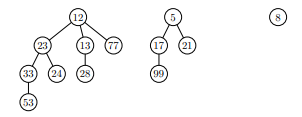
\includegraphics[]{binomial_heap.PNG}
  \label{binomial-heap}
\end{model*}

How many total nodes does the binomial heap in Model \ref{binomial-heap} contain?

\item What is the order of each binomial tree in Model \ref{binomial-heap}?

\item The table in Model \ref{heaptrees} lists a total number of nodes and the number of trees of each order. Fill in the table.

\begin{model*}{Trees in binomial heap of size $n$}{heaptrees}
  \centering
  % \tabcolsep=0.1cm
  \begin{tabular}{c|cccccccccccccccc}
    $n$ & $0$ & $1$ & $2$ & $3$ & $4$ & $5$ & $6$ & $7$ & $8$ & $9$ & $10$
    & $11$ & $12$ & $13$ & $14$ & $15$  \\[8pt]
    Order 0 trees & $0$ & $1$ & $0$ & & & & & & & & & & & & & \\[8pt]
    Order 1 trees & $0$ & $0$ & $1$ & & & & & & & & & & & & & \\[8pt]
    Order 2 trees & $0$ & $0$ & $0$ & & & & & & & & & & & & & \\[8pt]
    Order 3 trees & $0$ & $0$ & $0$ & & & & & & & & & & & & & \\[8pt]
  \end{tabular}
  \label{heaptrees}
\end{model*}

\item What is the relationship between the number of elements in a binomial heap and the orders of the binomial trees that it contains?

\item If a binomial heap has a total of $n$ elements, what is the maximum number of binomial trees that it contains? 

\item The \verb|merge| operation takes two binomial heaps as parameters and returns a new binomial heap containing all of the values from the first two heaps. If two binomial heaps each have one tree of order 0, explain how \verb|merge| will create a new binomial heap.

\item Next, imagine that we want to \verb|merge| two binomial heaps, one of which has an order 0 binomial tree, the other of which has an order 1 binomial tree. Explain how \verb|merge| will create a new binomial heap.

\item Now imagine that we want to \verb|merge| two binomial heaps, each of which has an order 0 binomial tree and also an order 1 binomial tree. Explain how \verb|merge| will create a new binomial heap.

\item Based on the insights gained from the previous three questions, write pseudocode for \verb|merge|.

\item What is the relationship between the \verb|merge| algorithm and the binary counter from the \emph{Introduction to Amortized Analysis} POGIL activity? \label{counter}

\item What is the best-case execution time for one call to \verb|merge|?

\item What is the worst-case execution time for one call to \verb|merge|?

\item What is the worst-case amortized execution time for $n$ calls to \verb|merge|? Feel free to use your answer to Question \ref{counter} to support your answer to this question. \label{amortizedN}

\item Based on your answer to Question \ref{amortizedN}, what is the worst-case amortized execution time for one call to \verb|merge|?

\item Priority queues have three main operations:
\begin{itemize}
    \item INSERT: Insert a new value into the heap.
    \item FIND-MIN: Find the smallest value in the heap.
    \item DELETE-MIN: Remove the smallest value from the heap.
\end{itemize}

Devise an algorithm for INSERT that uses \verb|merge| as a subroutine. 

\item What is the amortized worst-case execution time for INSERT?

\item Devise an algorithm for DELETE that uses \verb|merge| as a subroutine. 

\item What is its worst-case execution time for DELETE?

\item Devise a constant-time algorithm for FIND-MIN. You may want to make a small modification to the binomial heap data structure to ensure that it runs in constant time.

\item What advantages does a binomial heap have in comparison to the standard binary heap?

\item What advantages does a standard binary heap have in comparison to a binomial heap?

\end{questions}

\end{document}